\documentclass[conference]{IEEEtran}
% If the IEEEtran.cls has not been installed into the LaTeX system files, 
% manually specify the path to it:
% \documentclass[conference]{../sty/IEEEtran} 
\usepackage[brazil]{babel}
\usepackage{amsmath}
\usepackage{multirow}
\usepackage[utf8]{inputenc}
\usepackage[T1]{fontenc}
\usepackage{graphicx}
\usepackage{adjustbox}
\usepackage{booktabs}

% correct bad hyphenation here
\hyphenation{op-tical net-works semi-conduc-tor IEEEtran}

\begin{document}
	
	% paper title
	\title{Avaliação de Classificadores utilizando Técnicas de Estimativa de Densidades}
	
	
	% author names and affiliations
	% use a multiple column layout for up to three different
	% affiliations
	\author{\authorblockN{Victor São Paulo Ruela \\}
		\authorblockA{Programa de Pós-Graduação em Engenharia Elétrica\\
			Universidade Federal de Minas Gerais\\
			Belo Horizonte, Brasil\\
            Email: victorspruela@ufmg.br}}
	
	% avoiding spaces at the end of the author lines is not a problem with
	% conference papers because we don't use \thanks or \IEEEmembership
	
	% use only for invited papers
	%\specialpapernotice{(Invited Paper)}
	
	% make the title area
	\maketitle
	
	\begin{abstract}
		A modelagem de dados não-lineares com redes neurais artificiais depende da qualidade projeção aplicada sobre as entradas, geralmente feita através de funções de kernel. A otimização de seus parâmetros é uma etapa importante e pode ser feita via técnicas de estimativa de densidade. Além de fornecer uma forma automática de seleção dos parâmetros ótimos, estas técnicas possuem a tendência de gerar projeções ortogonais das entradas no espaço de projetado. A partir desta observação, este trabalho tem como objetivo avaliar o desempenho de classificadores lineares sobre esta projeção, considerando problemas de benchmark presentes na literatura. 
	\end{abstract}

	\section{Introdução}
	
	O desempenho de redes neurais artificiais sobre dados não-lineares é altamente dependente da projeção aplicada sobre as entradas, geralmente feita através de kernels. Estas funções possuem diversos parâmetros a serem ajustados, os quais irão afetar diretamente a qualidade do modelo obtido. O ajuste de seus paramêtros é geralmente realizado via técnicas de busca exaustiva, como validação cruzada~\cite{cortes1995support}. Embora amplamente utilizadas, tais técnicas não utilizam informações presentes nos dados. Isso motivou o desenvolvimento de, por exemplo, técnicas baseadas em estimativa de densidade para analisar a estrutura dos dados e reduzir a necessidade de interação do usuário~\cite{menezes2019width}. 
	
	Baseado no KDE (\textit{Kernel Density Estimation})~\cite{wang2013gaussian}, esta abordagem exploram o comportamento da projeção das funções de similaridade calculadas sobre kernel escolhido. É determinada uma função sobre os parâmetros do kernel, a qual pode ser utilizada para determinar os parâmetros que melhor se ajustam aos dados. É possível, por exemplo, usar este conceito para a determinação da largura ótima de kernels radiais (RBF) para o algoritmo SVM~\cite{menezes2019width}. Um resultado importante desta técnica está no fato dela poder gerar projeções ortogonais no espaço de verossimilhanças. Isso sugere a possibilidade de utilizar modelos lineares sobre esta projeção, como o Perceptron e aprendizado Hebbiano.
	
	Este trabalho tem como objetivo avaliar o desempenho dos modelos Perceptron simples \cite{rosenblatt1957perceptron} e Hebbiano~\cite{fernandez2011direct} sobre as projeções no espaço de verossimilhanças. Serão considerados tanto os kernels gaussiano e perceptron de múltiplas camadas (MLP), disponibilizados pelo professor. Além destes modelos, serão considerados também o ELM com regularização~\cite{huang2004extreme}, SVM~\cite{menezes2017otimizaccao, menezes2019width} e RBF com otimização de largura, aplicados sobre o espaço das entradas. Este último modelo não possui publicação associada e é proposto como forma de extensão ao enunciado original do trabalho. 
	Um experimento será desenhado para compará-los estatisticamente sobre diferentes bases de dados de \textit{benchmark} disponíveis na literatura. 
	

	\section{Revisão da literatura}

	\subsection{Métodos baseados em Kernel}
	
	
	
%	\subsection{Redes RBF}
%	As redes RBF foram inicialmente introduzidas por~\cite{broomhead1988multivariablefi} e são caracterizadas por um aprendizado que envolve duas etapas: (i) aplicar uma transformação aos padrões para um espaço onde a probabilidade de serem linearmente separáveis é alta (ii) encontrar os pesos usando o estimador mínimos quadrados usado no Perceptron simples. Essa estrutura pode ser representada por um rede de três camadas, onde sua camada escondida é reponsável pela transformação não-linear das entradas para o novo espaço, geralmente para uma dimensão muito alta. 
%	
%	Essa transformação é justificada pelo teorema de Cover sobre a separabilidade de padrões~\cite{cover1965geometrical}, o qual diz que um problema de classificação complexo projetado não-linearmente para um espaço de alta dimensão é mais provável de ser separável do que em um espaço de baixa dimensão, desde que o espaço não seja densamente povoado. Boa parte da teoria, que é relacionada ao campo de interpolação multivariável, considera um kernel baseado na função Gaussiana, que é uma classe importante de RBFs. Teoricamente, as redes RBF podem ser consideradas um aproximador universal de funções contínuas se a RBF é selecionada apropriadamente~\cite{poggio1990networks, park1991universal, liao2003relaxed}.
%	
%	\subsection{ELM}	
%	Inicialmente proposto por~\cite{huang2004extreme}, as máquinas de aprendizado extremo (ELM) são redes neurais com uma única camada escondida, as quais possuem o atrativo de poucos parâmetros a serem ajustados, generalização maior ou similar e redução do tempo de treinamento das redes em relação aos métodos convencionais. Seu treinamento é baseado na teoria de minimização de risco empírico, necessitando de somente uma iteração para este processo, evitando múltiplas iterações e algoritmos de otimização local~\cite{ding2015extreme}. 
%	
%	ELMs são capazes de definir adaptivamente o número neurônios da rede e aleatoriamente escolher os pesos das entradas e viéses da camada escondida~\cite{huang2006extreme}. Isso faz com o que a rede possa ser considerada como um sistema linear, o qual pode ser calculado de forma analítica através de uma operação de inversão da matriz de pesos da camada de saídas~\cite{huang2006extreme}. Essa característica permite uma drástica redução do esforço computacional do treinamento, geralmente de 10 vezes ou mais~\cite{deng2010research}. 
	
	\section{Metodologia}
	\subsection{Bases de Dados}
	Neste trabalho serão consideradas quinze bases de dados referentes a problemas de classificação binários disponíveis no repositório da UCI~\cite{dua2019}. Antes do treinamento, os dados de entrada serão normalizados para o intervalo $[0,1]$ e filtrados para remoção de valores inválidos. Um sumário das bases de dados consideradas pode ser vista na Tabela \ref{tab:datasets}.

	\begin{table}[h!]
		\centering
		\label{tab:datasets}
		\begin{tabular}{|l|c|c|c|}
			\hline
			\multicolumn{1}{|c|}{\textbf{Dataset}} & \textbf{Instâncias} & \textbf{Atributos} & \textbf{Proporção} \\ \hline
			ILPD                                   & 578                 & 10                 & 0.71/0.29          \\ \hline
			appendicitis                           & 106                 & 7                  & 0.80/0.20          \\ \hline
			australian                             & 690                 & 14                 & 0.56/0.44          \\ \hline
			banknote                               & 1372                & 4                  & 0.56/0.44          \\ \hline
			breastcancer                           & 569                 & 30                 & 0.37/0.63          \\ \hline
			bupa                                   & 345                 & 6                  & 0.42/0.58          \\ \hline
			climate                                & 540                 & 18                 & 0.09/0.91          \\ \hline
			fertility                              & 100                 & 9                  & 0.88/0.12          \\ \hline
			glass                                  & 214                 & 9                  & 0.86/0.14          \\ \hline
			haberman                               & 306                 & 3                  & 0.74/0.26          \\ \hline
			heart                                  & 270                 & 13                 & 0.56/0.44          \\ \hline
			ionosphere                             & 351                 & 33                 & 0.64/0.36          \\ \hline
			sonar                                  & 208                 & 60                 & 0.47/0.53          \\ \hline
			segmentation                           & 2310                & 19                 & 0.86/0.14          \\ \hline
			pima                                   & 768                 & 8                  & 0.65/0.35          \\ \hline
		\end{tabular}
	\end{table}

	\subsection{Desenho do experimento}
	A partir das recomendações para desenho de experimento para comparação de algoritmos proposta em~\cite{salzberg1997comparing}, a seguinte metodologia será adotada:
	\begin{itemize}
		\item Para cada base de dados:
			\begin{enumerate}
			\item Particionar os dados $D$ em $k$ partições para validação cruzada, mantendo a mesma proporção entre os rótulos
			\begin{enumerate}
				\item Criar o conjunto de treino $T = D - k$
				\item Para cada modelo:
				\begin{enumerate}
					\item Executar busca exaustiva com validação cruzada de $z$ partições sobre $T$ para os coeficientes de regularização $\lambda$ \label{item:grid-search}
					\item Escolher $\lambda$ que obtém o melhor ajuste médio 
					\item Avaliar a métrica do modelo sobre $k$
				\end{enumerate}
			\end{enumerate}
			\item Estimar o intervalo de confiança de 95\% do valor médio da métrica sobre $k$ usando \textit{bootstraping}
		\end{enumerate}
	\end{itemize}
	
	O número de partições consideradas será de $k=10$. Para o item \ref{item:grid-search}, serão considerados um número fixo de valores igualmente espaçados dentro de um intervalo pré-definido. Além disso, serão considerados $z=5$ partições, como forma de controlar um pouco o tamanho do experimento. Serão consideradas as acurácia como a métrica para comparação dos algoritmos. A implementação deste experimento, bem como dos modelos utilizados, será feita em Python e utilizando principalmente os pacotes \textit{numpy}~\cite{harris2020array} e \textit{scikit-learn}~\cite{scikit-learn}. O experimento será realizado em um Notebook Intel Core i7 Quad Core com 8Gb de memória RAM, sendo que o uso de paralelização será utilizado sempre que possível visto a enorme quantidade de vezes que os modelos serão treinados.
	
	\subsection{Aprendizado Hebbiano}
	O uso de aprendizado Hebbiano após a camada escondida é uma abordagem simples e eficiente para se controlar a generalização do modelo. Conforme sugerido em~\cite{horta2015aplicaccao}, podemos substituir o cálculo da pseudo-inversa da matriz de projeção, o que caracteriza a regra de aprendizado do Percepton simples, por um Perceptron Hebbiano com pesos normalizados. Essa abordagem é melhor descrita em~\cite{fernandez2011direct}, da qual podemos retirar a seguinte regra para problemas de classificação binários:
	\begin{equation}
		w = \frac{ \sum^{N}_{i=1} y_i\textbf{h}_i}{\left\|  \sum^{N}_{i=1} y_i\textbf{h}_i \right\| }
	\end{equation}
	onde $\textbf{h}_i$ é á $i$-ésima linha da matriz de projeção. É importante ressaltar que esta regra assume que os dados foram normalizados para possuir média zero e desvio padrão unitário. Conforme os resultados obtidos no anterior da disciplina, o uso do aprendizado Hebbiano é capaz de atingir a regularização desejada, porém seu desempenho é limitado a projeções que tornam os dados linearmente separáveis. Logo, podemos concluir que esta abordagem poderá ter desempenho satisfatório caso a projeção no espaço de verossimilhanças seja ortogonal.
	
	\subsection{RBF com Otimização de Largura}
	As redes RBF foram inicialmente introduzidas por~\cite{broomhead1988multivariablefi} e são caracterizadas por um aprendizado que envolve duas etapas: (i) aplicar uma transformação aos padrões através de um kernel Gaussiano (ii) encontrar os pesos usando o estimador mínimos quadrados usado no Perceptron simples. Portanto, a qualidade do modelo obtido será diretamente afetado pela escolha dos centróides e larguras das funções radias de cada neurônios. 
	
	Esta definição é geralmente feita utilizando o algotimo \textit{k-means} \cite{haykin2007neural}, porém podemos facilmente ver que a mesma abordagem de otimização da largura de SVMs com kernel RBF proposta por~\cite{menezes2019width} pode ser aplicada. Se considerarmos que cada neurônio usará a largura ótima obtida pela técnica anterior, precisamos definir somente os centróides na sequência, os quais serão amostrados uniformemente no espaço de entradas, resultando em um menor esforço computacional e complexidade. Na etapa final de treinamento, também será feito o uso de regularização para um maior controle de sua generalização. Espera-se um desempenho similar ao SVM, porém sem a expectativa de maximização de margem durante o treinamento, a qual será controlada pelo coeficiente de regularização.
	
	\section{Resultados}
	Os classificadores avaliados serão identificados por: \textbf{GK-H}, \textbf{GK-P}, \textbf{MLPK-H}, \textbf{MLPK-P}, \textbf{GK-SVM} e \textbf{GK-RBF}. Os prefixos \textbf{GK} e \textbf{MLPK} representam a projeção utilizada no espaço de verossimilhanças: kernel Gaussiano e MLP, respectivamente. Os sufixos \textbf{H}, \textbf{P}, \textbf{SVM} e \textbf{RBF} representam o modelo utilizado: Perceptron Hebbiano, Perceptron Simples, SVM e RBF respectivamente.
	
	\subsection{Análise de problemas bi-dimensionais}
	Considerando três conjuntos de dados gerados artificialmente para diferentes estruturas, a superfície de decisão para cada classificador pode ser vista nas Figuras \ref{fig:ds01_circles}, \ref{fig:ds02_quant} e \ref{fig:ds03_spirals}. Observe que à medida em que a complexidade do modelo é aumentada, maior é a dificuldade encontrada pelos modelos lineares. 
	
	Para o problema da Figura \ref{fig:ds01_circles}, é possível ver que todos os modelos estimaram com precisão a superfície de separação. Entretanto, note que para o problema da Figura \ref{fig:ds02_quant} os modelos lineares não tiveram um bom desempenho, provavelmente devido à qualidade da projeção obtida. Isso é evidenciado pelo problema da Figura \ref{fig:ds03_spirals}, para o qual os modelos lineares obtiveram desempenho superior quando utilizada a projeção MLP. Destaca-se também que o RBF se ajustam muito bem aos dados e e de foram bem similar ao SVM, indicando que a estratégia adotada é bastante promissora.
	
	
	\begin{figure}[thpbh]
		\centering
		\includegraphics[width=0.5\textwidth]{figures/ds01_circles.png}
		\caption{Superfície de decisão para o problema de círculos concêntricos}
		\label{fig:ds01_circles}
	\end{figure}
	\begin{figure}[thpbh]
		\centering
		\includegraphics[width=0.5\textwidth]{figures/ds02_quant.png}
		\caption{Superfície de decisão para o problema de dois círculos concêntricos alternados}
		\label{fig:ds02_quant}
	\end{figure}
	\begin{figure}[thpbh]
		\centering
		\includegraphics[width=0.5\textwidth]{figures/ds03_spirals.png}
		\caption{Superfície de decisão para o problema das espirais}
		\label{fig:ds03_spirals}
	\end{figure}

	\subsection{Análise do experimento}

	Considerando os mesmos algoritmos da seção anterior, é incluído também o algoritmo ELM com regularização na sua versão original, ou seja, sem o uso da técnica de projeção no espaço de verossimilhanças. O número de neurônios das redes ELM e GK-RBF foram mantidos fixos em 100. Os valores de coeficiente de regularização utilizados para o GK-SVM, RBF e ELM foram escolhidos no intervalo $[2^{-5},2^{-4}, \dots, 2^{11},2^{12}]$. A acurácia média e seu intervalo de confiança obtido via bootstraping para o experimento estão consolidados na Tabela \ref{tab:results}. Comparando com os resultados reportados em \cite{menezes2019width}, nota-se que todos estão coerentes, especialmente para a implementação do GK-SVM. Destaca-se o excelente desempenho do algoritmo ELM, o qual também está de acordo com o reportado na literatura \cite{huang2011extreme}.
	
	Observando os demais métodos avaliados, é importante destacar também que o modelo GK-RBF apresentou desempenho equivalente ao GK-SVM em grande parte das bases de dados, porém ainda com ma acurácia elevada e compatível com o esperado para a base de dados. Portanto, podemos afirmar que esta é uma abordagem que, embora simples de entender e implementar, tem potencial para novas aplicações. Embora a versão clássica do treinamento de redes RBF não foi incluída para comparação, uma outra vantagem que ficou evidente durante a execução do experimento foi a redução drástica no tempo de treinamento, uma vez que foi eliminada a necessidade do cálculo dos centros e raios via clustering.  
	
	A grande surpresa destes testes está na baixa qualidade dos resultados do modelo com aprendizado Hebbiano: para todas as bases de dados avaliadas, o modelo GK-H apresentou acurácia inferior em relação aos demais para um intervalo de confiança de 95\%. O mesmo não ocorreu quando foi utilizado o MLP-H, onde para algumas bases de dados a acurácia foi equivalente. Isso sugere que a projeção no espaço de verossimilhanças com o Kernel radial possa não ter atingido a ortogonalização esperada. 
	
	O cálculo do cross-talk sobre o conjunto de dados projetado permite obter uma ideia da qualidade desta ortogonalização, onde um valor próximo de zero indicará uma boa projeção. Os valores obtidos estão disponíveis na Tabela \ref{tab:crosstalk}, os quais foram calculados considerando a média do valor de cada amostra em relação à todas as outras. É relevante citar que durante o cálculo, se considerássemos somente as amostras de classes diferentes classe, o valor era aproximadamente zero e foram omitidos da tabela. Portanto, os valores apresentados correspondem ao cross-talk intra-classe, o qual é naturalmente mais alto. Dessa forma podemos concluir que a ortogonalização obtida é de fato ortogonal, e outro fator pode estar afetando o aprendizado Hebbiano.
	
	\begin{table}[h!]
		\centering
		\label{tab:crosstalk}
		\caption{Cross-talk calculado para as projeções RBF e MLP sobre todo o conjunto de dados}
		\begin{tabular}{|l|c|c|}
			\hline
			\multicolumn{1}{|c|}{\textbf{Dataset}} & \textbf{RBF} & \textbf{MLP} \\ \hline
			ILPD                                   & 0.973675     & 1.299812     \\ \hline
			appendicitis                           & 0.594261     & -1.086522    \\ \hline
			australian                             & 0.069242     & 0.029584     \\ \hline
			banknote                               & -0.212484    & -0.224532    \\ \hline
			breastcancer                           & 0.318198     & 0.575652     \\ \hline
			bupa                                   & -0.262322    & -1.124887    \\ \hline
			climate                                & -1.525012    & -1.253363    \\ \hline
			fertility                              & 1.445575     & 0.590236     \\ \hline
			glass                                  & -0.216374    & -1.345287    \\ \hline
			haberman                               & 0.756672     & 0.193615     \\ \hline
			heart                                  & -0.070371    & -0.422381    \\ \hline
			ionosphere                             & 0.048857     & -0.723001    \\ \hline
			pima                                   & 0.408878     & -0.415799    \\ \hline
			segmentation                           & 1.377789     & 0.043600     \\ \hline
			sonar                                  & -0.560352    & 0.396350     \\ \hline
		\end{tabular}
	\end{table}

	\begin{table*}[thpbh]
		\caption{Acurácia média dos classificadores para intervalo de confiança de 95\%}
		\label{tab:results}
		\begin{adjustbox}{width=1\textwidth}
			
		\begin{tabular}{@{}cccccccc@{}}
			\toprule
			\textbf{Base}                               & \textbf{ELM}                             & \textbf{GK-H}                            & \textbf{GK-P}                            & \textbf{GK-RBF}                           & \textbf{GK-SVM}                             & \textbf{MLPK-H}                             & \textbf{MLPK-P}                             \\ \midrule
			\multicolumn{1}{|l|}{ILPD}         & \multicolumn{1}{l|}{\textbf{70.97 (69.82,72.20})} & \multicolumn{1}{l|}{52.95 (49.00,56.68)} & \multicolumn{1}{l|}{66.29 (63.18,69.65)} & \multicolumn{1}{l|}{\textbf{71.45 (71.01,71.92)}}  & \multicolumn{1}{l|}{\textbf{71.43 (70.94,71.96)}}    & \multicolumn{1}{l|}{60.77 (55.69,66.12)}    & \multicolumn{1}{l|}{\textbf{71.43 (70.90,72.02)}}    \\ \midrule
			\multicolumn{1}{|l|}{appendicitis} & \multicolumn{1}{l|}{\textbf{85.82 (81.09,90.00)}} & \multicolumn{1}{l|}{76.36 (66.45,86.37)} & \multicolumn{1}{l|}{\textbf{87.64 (82.00,93.46)}} & \multicolumn{1}{l|}{\textbf{84.73 (78.00,90.91)}}  & \multicolumn{1}{l|}{\textbf{86.73 (80.36,92.55)}}    & \multicolumn{1}{l|}{61.55 (49.99,74.28)}    & \multicolumn{1}{l|}{75.36 (70.91,80.64)}    \\ \midrule
			\multicolumn{1}{|l|}{australian}   & \multicolumn{1}{l|}{85.94 (83.04,89.13)} & \multicolumn{1}{l|}{86.09 (83.33,88.99)} & \multicolumn{1}{l|}{87.60 (85.35,89.70)} & \multicolumn{1}{l|}{86.09 (83.62,89.13)}  & \multicolumn{1}{l|}{85.80 (82.90,88.84)}    & \multicolumn{1}{l|}{85.19 (82.93,87.60)}    & \multicolumn{1}{l|}{83.91 (81.88,85.95)}    \\ \midrule
			\multicolumn{1}{|l|}{banknote}    & \multicolumn{1}{l|}{\textbf{97.96 (97.45,98.54)}} & \multicolumn{1}{l|}{91.76 (90.44,93.08)} & \multicolumn{1}{l|}{91.91 (90.38,93.30)} & \multicolumn{1}{l|}{\textbf{99.78 (99.56,100.00)}} & \multicolumn{1}{l|}{\textbf{100.00 (100.00,100.00)}} & \multicolumn{1}{l|}{\textbf{100.00 (100.00,100.00)}} & \multicolumn{1}{l|}{\textbf{100.00 (100.00,100.00)}} \\ \midrule
			\multicolumn{1}{|l|}{breastcancer} & \multicolumn{1}{l|}{\textbf{96.48 (95.42,97.70)}} & \multicolumn{1}{l|}{92.09 (89.99,94.02)} & \multicolumn{1}{l|}{94.53 (93.74,95.31)} & \multicolumn{1}{l|}{91.21 (90.33,92.09)}  & \multicolumn{1}{l|}{\textbf{98.82 (98.04,99.62)}}    & \multicolumn{1}{l|}{\textbf{96.88 (96.30,97.26})}    & \multicolumn{1}{l|}{\textbf{96.31 (94.91,97.54)}}    \\ \midrule
			\multicolumn{1}{|l|}{bupa}        & \multicolumn{1}{l|}{\textbf{70.45 (67.33,73.45)}} & \multicolumn{1}{l|}{50.14 (45.03,55.31)} & \multicolumn{1}{l|}{60.65 (58.71,62.75)} & \multicolumn{1}{l|}{61.10 (57.97,63.86)}  & \multicolumn{1}{l|}{\textbf{70.81 (65.53,76.24)}}    & \multicolumn{1}{l|}{55.96 (51.24,60.89)}    & \multicolumn{1}{l|}{57.10 (53.28,60.34)}    \\ \midrule
			\multicolumn{1}{|l|}{climate}      & \multicolumn{1}{l|}{\textbf{91.11 (90.37,91.67)}} & \multicolumn{1}{l|}{57.59 (54.81,60.00)} & \multicolumn{1}{l|}{\textbf{91.48 (90.93,92.04)}} & \multicolumn{1}{l|}{\textbf{91.11 (90.37,91.85)}}  & \multicolumn{1}{l|}{\textbf{91.30 (90.74,91.85)}}    & \multicolumn{1}{l|}{78.15 (70.37,87.04)}    & \multicolumn{1}{l|}{\textbf{89.81 (88.52,91.11)}}    \\ \midrule
			\multicolumn{1}{|l|}{fertility}    & \multicolumn{1}{l|}{\textbf{86.00 (83.00,89.00)}} & \multicolumn{1}{l|}{52.22 (42.22,61.14)} & \multicolumn{1}{l|}{\textbf{86.00 (83.00,89.00)}} & \multicolumn{1}{l|}{\textbf{87.78 (85.56,90.00)}}  & \multicolumn{1}{l|}{\textbf{87.00 (84.00,90.00)}}    & \multicolumn{1}{l|}{60.00 (50.00,70.00)}    & \multicolumn{1}{l|}{\textbf{87.78 (85.56,91.11)}}    \\ \midrule
			\multicolumn{1}{|l|}{glass}        & \multicolumn{1}{l|}{\textbf{96.26 (94.37,98.48)}} & \multicolumn{1}{l|}{86.84 (79.99,94.32)} & \multicolumn{1}{l|}{\textbf{97.08 (95.35,98.32)}} & \multicolumn{1}{l|}{\textbf{97.68 (95.84,99.94)}}  & \multicolumn{1}{l|}{\textbf{96.26 (93.90,99.05)}}    & \multicolumn{1}{l|}{\textbf{95.30 (92.49,98.61)}}    & \multicolumn{1}{l|}{\textbf{96.26 (93.94,98.55)}}    \\ \midrule
			\multicolumn{1}{|l|}{haberman}     & \multicolumn{1}{l|}{\textbf{76.24 (74.43,77.98)}} & \multicolumn{1}{l|}{53.59 (50.04,57.03)} & \multicolumn{1}{l|}{\textbf{74.69 (73.27,76.10)}} & \multicolumn{1}{l|}{\textbf{72.23 (70.04,74.55)}}  & \multicolumn{1}{l|}{\textbf{72.56 (71.01,74.11)}}    & \multicolumn{1}{l|}{52.57 (44.63,60.08)}    & \multicolumn{1}{l|}{\textbf{72.54 (71.30,74.05)}}    \\ \midrule
			\multicolumn{1}{|l|}{heart}        & \multicolumn{1}{l|}{\textbf{84.77 (83.54,86.01)}} & \multicolumn{1}{l|}{78.19 (74.48,82.30)} & \multicolumn{1}{l|}{\textbf{82.22 (78.52,85.56)}} & \multicolumn{1}{l|}{\textbf{85.19 (82.59,87.78)}}  & \multicolumn{1}{l|}{79.63 (76.67,82.59)}    & \multicolumn{1}{l|}{\textbf{82.22 (78.52,85.93)}}    & \multicolumn{1}{l|}{\textbf{87.50 (84.25,90.28)}}    \\ \midrule
			\multicolumn{1}{|l|}{ionosphere}   & \multicolumn{1}{l|}{\textbf{88.31 (85.98,91.17)}} & \multicolumn{1}{l|}{70.08 (66.00,74.65)} & \multicolumn{1}{l|}{\textbf{87.00 (84.11,90.20)}} & \multicolumn{1}{l|}{\textbf{89.47 (85.14,93.22)}}  & \multicolumn{1}{l|}{\textbf{93.73 (91.17,96.32)}}    & \multicolumn{1}{l|}{\textbf{92.89 (90.63,95.14)}}    & \multicolumn{1}{l|}{93.17 (90.88,95.62)}    \\ \midrule
			\multicolumn{1}{|l|}{pima}         & \multicolumn{1}{l|}{\textbf{76.42 (74.18,78.51)}} & \multicolumn{1}{l|}{67.44 (65.56,69.13)} & \multicolumn{1}{l|}{\textbf{72.52 (69.45,75.45)}} & \multicolumn{1}{l|}{\textbf{75.91 (73.45,78.52)}}  & \multicolumn{1}{l|}{\textbf{77.74 (75.83,79.59)}}    & \multicolumn{1}{l|}{\textbf{75.52 (72.63,78.08)}}    & \multicolumn{1}{l|}{\textbf{76.77 (75.32,78.02)}}    \\ \midrule
			\multicolumn{1}{|l|}{segmentation} & \multicolumn{1}{l|}{\textbf{99.65 (99.48,99.83)}} & \multicolumn{1}{l|}{57.06 (54.93,59.18)} & \multicolumn{1}{l|}{\textbf{88.79 (87.97,89.65)}} & \multicolumn{1}{l|}{\textbf{98.61 (98.14,99.09)}}  & \multicolumn{1}{l|}{\textbf{99.70 (99.48,99.91)}}    & \multicolumn{1}{l|}{78.16 (75.71,80.42)}    & \multicolumn{1}{l|}{85.71 (85.71,85.71)}    \\ \midrule
			\multicolumn{1}{|l|}{sonar}        & \multicolumn{1}{l|}{77.14 (73.33,81.59)} & \multicolumn{1}{l|}{69.52 (65.55,73.81)} & \multicolumn{1}{l|}{75.06 (73.24,76.87)} & \multicolumn{1}{l|}{73.97 (70.63,77.62)}  & \multicolumn{1}{l|}{\textbf{86.19 (83.33,89.21)}}    & \multicolumn{1}{l|}{\textbf{81.27 (78.89,83.81)}}    & \multicolumn{1}{l|}{\textbf{80.48 (77.46,83.65)}}    \\
			\midrule
			\multicolumn{1}{|l|}{\textbf{Average}}        & \multicolumn{1}{l|}{\textbf{85.87 (84.26,87.61)}} & \multicolumn{1}{l|}{69.49 (67.11,72.01)} & \multicolumn{1}{l|}{\textbf{82.55 (81.04,84.29)}} & \multicolumn{1}{l|}{\textbf{84.94 (83.10,86.61)}}  & \multicolumn{1}{l|}{\textbf{86.66 (85.11,88.33)}}    & \multicolumn{1}{l|}{75.35 (72.56,78.27)}    & \multicolumn{1}{l|}{\textbf{83.76 (81.96,85.44)}} \\ \bottomrule
		\end{tabular}
		\end{adjustbox}
	\end{table*}


%	\begin{table*}[thpbh]
%		\caption{Intervalos de confiança de 95\% calculados para a AUC média}
%		\label{tab:classification}
%		\centering
%		\begin{tabular}{r|r|r|r|r|}
%			\cline{2-5}
%			\multicolumn{1}{l|}{}                          & \multicolumn{1}{c|}{\textbf{ELM}} & \multicolumn{1}{c|}{\textbf{ELM Hebbiano}} & \multicolumn{1}{c|}{\textbf{Perceptron}} & \multicolumn{1}{c|}{\textbf{RBF}} \\ \hline
%			\multicolumn{1}{|r|}{\textbf{Breast Cancer}}   & \textbf{0.948 (0.935,0.963)}         & 0.887 (0.853,0.920)                           & \textbf{0.950 (0.930,0.971)}                & 0.512 (0.505,0.519)                  \\ \hline
%			\multicolumn{1}{|r|}{\textbf{Liver Disorder}}  & \textbf{0.677 (0.621,0.733)}         & 0.582 (0.536,0.628)                           & 0.532 (0.509,0.553)                         & 0.515 (0.498,0.537)                  \\ \hline
%			\multicolumn{1}{|r|}{\textbf{Statlog (Heart)}} & \textbf{0.812 (0.769,0.851)}         & 0.762 (0.698,0.819)                           & 0.772 (0.700,0.846)                         & 0.547 (0.522,0.569)                  \\ \hline
%		\end{tabular}
%	\end{table*}


%	\begin{figure}[thpbh]
%		\centering
%		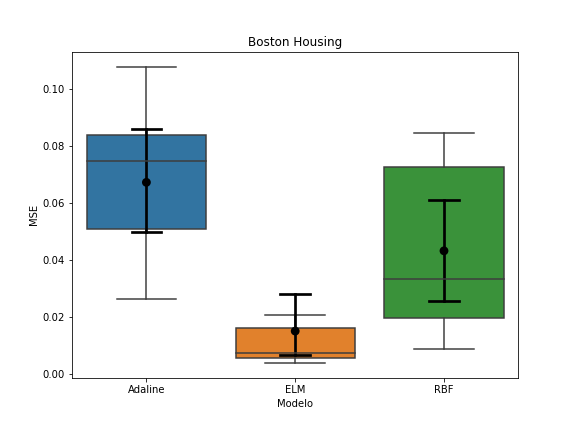
\includegraphics[width=0.5\textwidth]{figures/Boston Housing_scores.png}
%		\caption{Boxplots para a base de dados \textit{Boston Housing}. Intervalos de confiança de 95\% para a média são exibidos em preto.}
%		\label{fig:box-Boston-Housing}
%	\end{figure}
%	
%	\begin{figure}[thpbh]
%		\centering
%		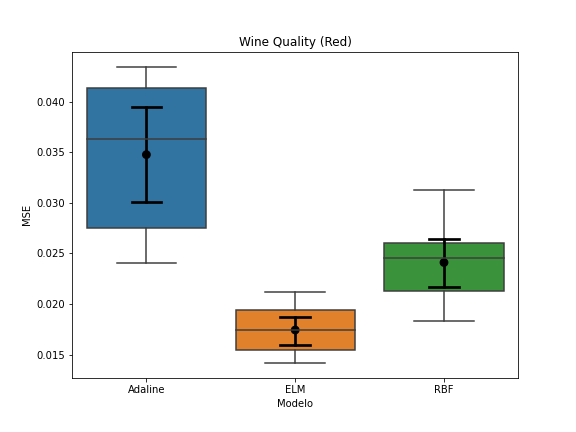
\includegraphics[width=0.5\textwidth]{figures/Wine Quality (Red)_scores.png}
%		\caption{Boxplots para a base de dados \textit{Wine Quality (Red)}. Intervalos de confiança de 95\% para a média são exibidos em preto.}
%		\label{fig:box-Wine}
%	\end{figure}
%	
%	\begin{figure}[thpbh]
%		\centering
%		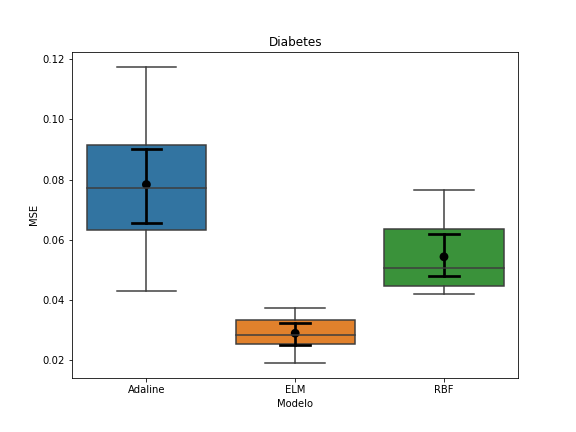
\includegraphics[width=0.5\textwidth]{figures/Diabetes_scores.png}
%		\caption{Boxplots para a base de dados \textit{Diabetes}. Intervalos de confiança de 95\% para a média são exibidos em preto.}
%		\label{fig:box-Diabetes}
%	\end{figure}


	
	\section{Conclusões}
	
	Neste trabalho foi feita uma avaliação do desempenho do ELM e modelos usando a abordagem por projeção no espaço de verossimilhanças sobre bases de dados de benchmark presentes na literatura. A partir de um experimento desenhado para tal finalidade, os resultados foram comparados estatísticamente utilizando a técnica de \textit{bootstrapping} para a acurácia média, considerando um intervalo de confiança de 95\%. Destaca-se o excelente desempenho do ELM em todos os conjuntos de dados, conforme observado nos trabalhos anteriores. É importante destacar também que resultados compatíveis com a literatura foram obtidos para o SVM com otimização da largura. Além disso, a aplicação deste mesmo conceito para o treinamento de redes RBF se mostrou bastante eficaz. Notou-se também que os modelos lineares avaliados obtiveram bons resultados dependendo da base de dados em questão, conseguindo atingir um desempenho estatisticamente equivalente aos demais.
	
	Assim como no trabalho anterior, o desempeho do aprendizado Hebbiano deixou a desejar, apresentando um resultado muito inferior em relação aos demais modelos. Uma avaliação do cross-talk das bases de dados mostrou que não houve uma correlação clara entre o seu aumento e a baixa acurácia do modelo, de forma a indicar que outro fator esteja causando este problema. Para algumas bases de dados ele consegue atingir uma acurácia alta, embora estatisticamente tenha ficado inferior aos demais métodos para um intervalo de confiança de 95\%.
	
	Como trabalhos futuros, é sugerido uma investigação mais detalhada do que pode estar causando a baixa acurácia dos modelos com aprendizado Hebbiano. Além disso, seria interessante incluir o modelo RBF com aprendizdo via clustering e compará-lo com o novo método proposto. 
		


    \bibliographystyle{unsrt}
	\bibliography{artigo3}
	
\end{document} 